\documentclass[11pt]{article}

%Sonderzeichen
\usepackage[T1]{fontenc}
\usepackage[utf8x]{inputenc} 

%Bilder
\usepackage{graphicx}
\usepackage{subfigure}
%Bild bennenen
\renewcommand{\figurename}{Bild}
%Nach Bild einrücken
\setlength{\parindent}{0pt}

%Stichwortverzeichnis
\usepackage{makeidx}
\makeindex

%Ränder
\usepackage{anysize}
\marginsize{2.4cm}{2.4cm}{2.2cm}{3cm}


%Sprache
\usepackage[german]{babel}
%\select@language{german}

%Numerierungstiefe
\setcounter {secnumdepth}{3}
\setcounter{tocdepth}{2}

%Verzeichnis verlinken
\usepackage{hyperref}

%Farben (Inhaltsverzeichnis)
\usepackage{color}
\definecolor{black}{rgb}{0,0,0}
\hypersetup{colorlinks, linkcolor=black}


%Kopf und Fusszeilen
\usepackage{fancyhdr}
\pagestyle{fancy} %vordefinierter Style
\fancyhf{}
%Kopfzeile
\fancyhead[L]{\nouppercase{\leftmark}}
\fancyhead[C]{TG 13/3 Projektdokumentation}
\fancyhead[R]{\today}
\renewcommand{\headrulewidth}{0.5pt}
\headheight 15pt
%Fusszeile
\fancyfoot[L]{Fabian Zeller }
\fancyfoot[C]{\thepage}
\fancyfoot[R]{Emanuel Hubenschmidt}
\renewcommand{\footrulewidth}{0.0pt}
\footskip 63pt

%Tabellen

\usepackage{tabularx}
\usepackage{float}
\floatplacement{figure}{H}

%Literaturverzeichnis
\usepackage{url}
\usepackage{cite}
\hypersetup{colorlinks, linkcolor=black}

%Mathematisch
\usepackage{amssymb}

%Code einbinden
\usepackage{listings} 
\usepackage{color}   
\usepackage[svgnames]{xcolor} 

\definecolor{mygreen}{rgb}{0,0.6,0}
\definecolor{mygray}{rgb}{0.5,0.5,0.5}
\definecolor{mymauve}{rgb}{0.58,0,0.82}

\lstset{language=Java}
\lstset{ %
  backgroundcolor=\color{white},   % choose the background color; you must add \usepackage{color} or \usepackage{xcolor}
  basicstyle=\footnotesize,        % the size of the fonts that are used for the code
  breakatwhitespace=false,         % sets if automatic breaks should only happen at whitespace
  breaklines=true,                 % sets automatic line breaking
  captionpos=b,                    % sets the caption-position to bottom
  commentstyle=\color{mygreen},    % comment style
  deletekeywords={...},            % if you want to delete keywords from the given language
  escapeinside={\%*}{*)},          % if you want to add LaTeX within your code
  extendedchars=true,              % lets you use non-ASCII characters; for 8-bits encodings only, does not work with UTF-8
  frame=single,	                   % adds a frame around the code
  keepspaces=true,                 % keeps spaces in text, useful for keeping indentation of code (possibly needs columns=flexible)
  keywordstyle=\color{blue},       % keyword style
  language=Java,                   % the language of the code
  otherkeywords={*,...},           % if you want to add more keywords to the set
  numbers=left,                    % where to put the line-numbers; possible values are (none, left, right)
  numbersep=5pt,                   % how far the line-numbers are from the code
  numberstyle=\tiny\color{mygray}, % the style that is used for the line-numbers
  rulecolor=\color{black},         % if not set, the frame-color may be changed on line-breaks within not-black text (e.g. comments (green here))
  showspaces=false,                % show spaces everywhere adding particular underscores; it overrides 'showstringspaces'
  showstringspaces=false,          % underline spaces within strings only
  showtabs=false,                  % show tabs within strings adding particular underscores
  stepnumber=2,                    % the step between two line-numbers. If it's 1, each line will be numbered
  stringstyle=\color{mymauve},     % string literal style
  tabsize=2,	                   % sets default tabsize to 2 spaces
  title=Codeausschnitt                 % show the filename of files included with \lstinputlisting; also try caption instead of title
}



\begin{document}

%Deckblatt

\title{Projektarbeit 2016\\TwitterStego-App}
\author{F.Zeller\\E.Hubenschmidt}
\maketitle
\newpage

%Inhaltsverzeichnis
\tableofcontents
\newpage

\section{Funktionsweise und Beschreibung}

\subsection{Beschreibung}
Die TwitterStego-App ist ein Programm für den PC welches Nachrichten in Bildern verstecken und wieder herausfiltern kann. Des weiteren kann man diese Bilder auf Twitter tweeten und auch nach Bildern auf Twitter suchen. Das Programm dient also zur verstecken Kommunikation über Twitter.

\subsection{Funktionsweise}

\begin{figure}[hbtp]
\centering
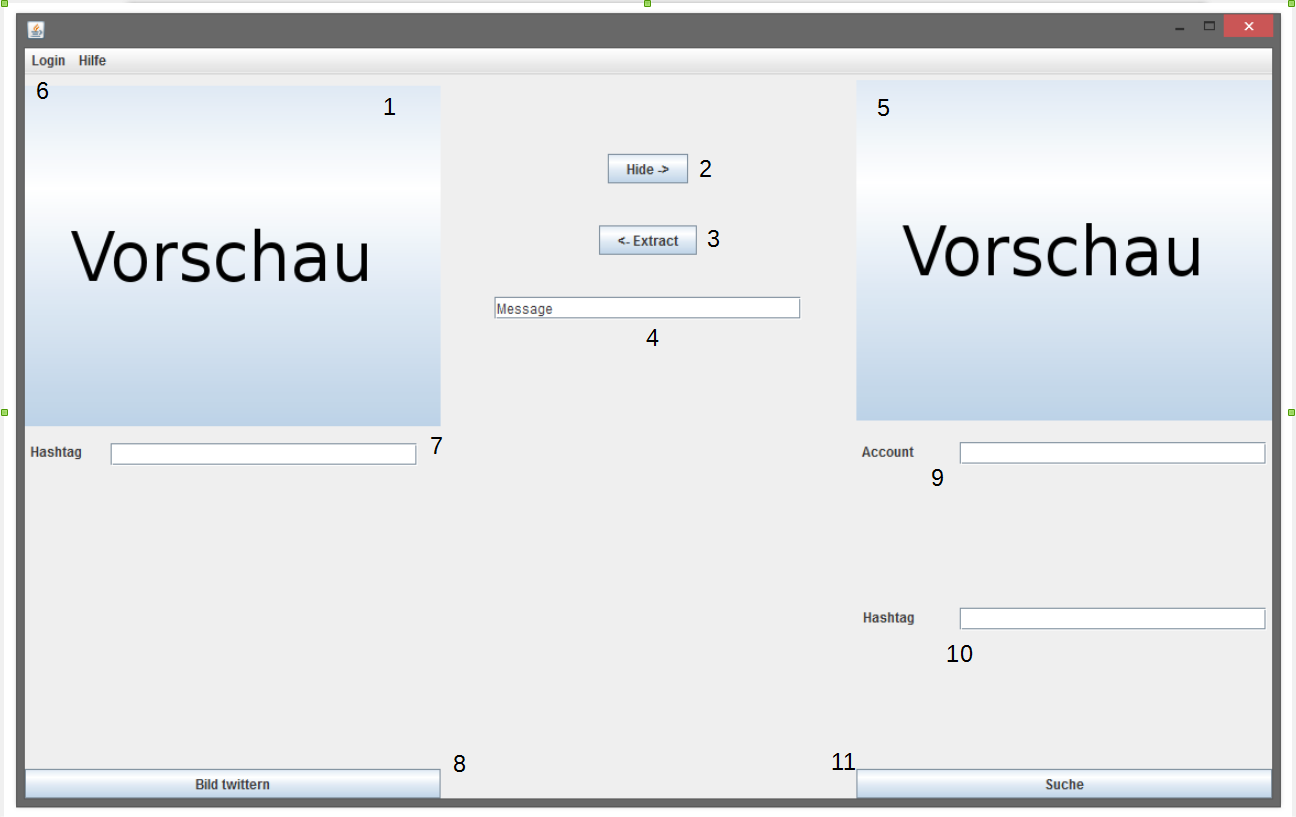
\includegraphics[scale=0.4]{GuiBeschriftet.PNG}
\caption{Die Oberfläche}
\end{figure}


\subsubsection{Nachrichten in Bildern verstecken}
Um eine Nachricht in einem Bild zu verstecken muss als erstes das Bild ausgewählt werden. Hierfür betätigt man die große Vorschau Fläche(1). Es öffnet sich ein Dateiexplorer und man kann ein Bild auswählen. Dieses Bild wird nun auf der Vorschaufläche angezeigt. 
\\
Als nächstes gibt man die zu versteckende Nachricht in das Message Feld(4) rechts neben der Vorschau ein. Um die Nachricht zu verstecken muss nur noch der Hide-Button(2) betätigt werden. Es öffnet sich wieder ein Dateiexplorer und man wählt den Speicherort für das Bild mit versteckter Nachricht aus.

\newpage

\subsubsection{Nachrichten aus Bildern filtern}
Um eine Nachricht aus einem Bild zu filtern muss das Bild ausgewählt werden. Hierfür betätigt man die rechte Vorschau Fläche(5). Mithilfe des Dateiexplorers wählt man das gewünschte Bild aus. Es erscheint nun in der rechten Vorschau. Sobald man den Extract-Button(3) betätigt wird die Nachricht im Message Feld(4) angezeigt. 

\subsubsection{Der Login}
Um auf Twitter zugreifen zu können muss man sich ersteinmal anmelden. Hierfür benötigt man den AccesToken, das AccesTokenSecret, den ConsumerKey sowie das ConsumerSecret. Diese vier Schlüsselbekommt man von Twitter. Man meldet sich hier: \url{https://apps.twitter.com/} mit seinem Twitter-Account an und folgt den Instruktionen. Sobald man seine Schlüssel hat wählt man in dem Menu Login(6) den Unterpunkt Neuer Login aus. Hier gibt man seine eben erworbenen Schlüssel sowie einen Speichername für diesen Login ein.
Ab sofort kann man auch die Twitterfunktionen der TwitterStego-App nutzen.


\subsubsection{Ein Bild Twittern}
Um ein Bild zu Twittern muss man nur einen beliebigen (optimal einen wenig oder nur eigen benutzten) Hashtag in das vorgesehene Feld(7) eintragen. Sobald der Button Bild-Twittern(8) betätigt wurde öffnet sich der Dateiexplorer und man kann das gewünschte Bild auswählen. 

\subsubsection{Ein Bild von Twitter suchen}




\newpage
\section{Steganographie}

Kryptographie\index{Krypto}



\newpage
\section{Entwicklungshergang}

\subsection{Zeitliches Limit}

Da das Schulprojekt auf nur 3 Wochen begrenzt war mussten wir uns bei der Gestaltung der TwitterStego-App beschränken. 





\subsection{Aufteilung der Aufgaben}


\newpage
\section{Reflexion}





%Stichwortverzeichniss
\newpage
\renewcommand{\indexname}{Stichwortverzeichnis}

% Stichwortverzeichnis Im Inhaltsverzeichniss
\addcontentsline{toc}{section}{Stichwortverzeichnis}

% Stichwortverzeichnis anzeigen
\printindex

\end{document}